% Copyright 2020-2022 Robert Bosch GmbH

% Licensed under the Apache License, Version 2.0 (the "License");
% you may not use this file except in compliance with the License.
% You may obtain a copy of the License at

% http://www.apache.org/licenses/LICENSE-2.0

% Unless required by applicable law or agreed to in writing, software
% distributed under the License is distributed on an "AS IS" BASIS,
% WITHOUT WARRANTIES OR CONDITIONS OF ANY KIND, either express or implied.
% See the License for the specific language governing permissions and
% limitations under the License.

\hypertarget{webapp-architecture}{%
\section{TestResultWebApp Architecture}\label{webapp-architecture}}

The TestResultWebApp application includes:
\begin{itemize}
   \item Database: \href{https://mysql.com/}{MySQL} - which contains all test execution 
         results. For details of all tables in the database, please refer the 
         \href{https://github.com/test-fullautomation/testresultwebapp/blob/develop/TestResultWebApp/mysql_server/datamodel/datamodel.svg}{database
         model}.
   \item Active Directory: for the authentication.
   \item Web server: which hosts the static data and runs the \href{https://nodejs.org/}{Node.js}
         application for providing the dynamic data.
   \item Web client: is written in javascript which also use some libraries such 
         as \href{https://jquery.com/}{jQuery}, \href{https://getbootstrap.com/docs/5.0/getting-started/introduction/}{bootstrap},
         \href{https://www.chartjs.org/}{Chart.js}, 
         \href{https://d3js.org/}{D3} for data visualization. 
\end{itemize}

Please refer below architecture for more detail:

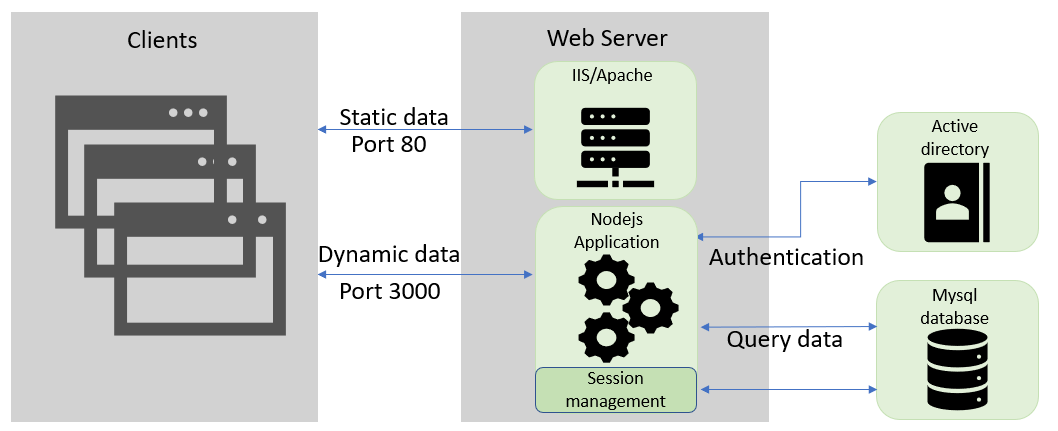
\includegraphics[width=1\linewidth]{./pictures/Architechture.png}

\hypertarget{import-data}{%
\section{Import Data}\label{import-data}}

The data which will be visualized on WebApp comes directly from the database.
For this the test execution result data must be transformed first 
into the defined \href{https://github.com/test-fullautomation/testresultwebapp/blob/develop/TestResultWebApp/mysql_server/datamodel/datamodel.svg}{database model} 
then imported into the database.

The data base model is generic, so test result data can be any. Only a test 
result importer must transfrom and import the data.

We provide already the \href{https://github.com/test-fullautomation/robotframework-testresultwebapptool}{RobotResults2DB}
which helps to import the \rfwcore\ result file(s) \emph{output.xml} to the 
database of the TestResultWebApp.

You will need to provide only the \rfwcore\ result file(s) and database's 
credential information, that RobotResults2DB will parse the test execution result data 
and interact with the provided database to import the data.

Please refer \href{https://github.com/test-fullautomation/robotframework-testresultwebapptool#usage}{RobotResults2DB's usage} and 
\href{https://github.com/test-fullautomation/robotframework-testresultwebapptool/blob/develop/RobotResults2DB/RobotResults2DB.pdf}
{its document} for more detail.


\hypertarget{data-visualization}{%
\section{Data Visualization}\label{data-visualization}}

\hypertarget{main-menu}{%
\subsection{Main menu}\label{main-menu}}
The WebApp provides a main menu for selecting a specific \textbf{branch}, 
\textbf{project/variant} and \textbf{software version} to be displayed.

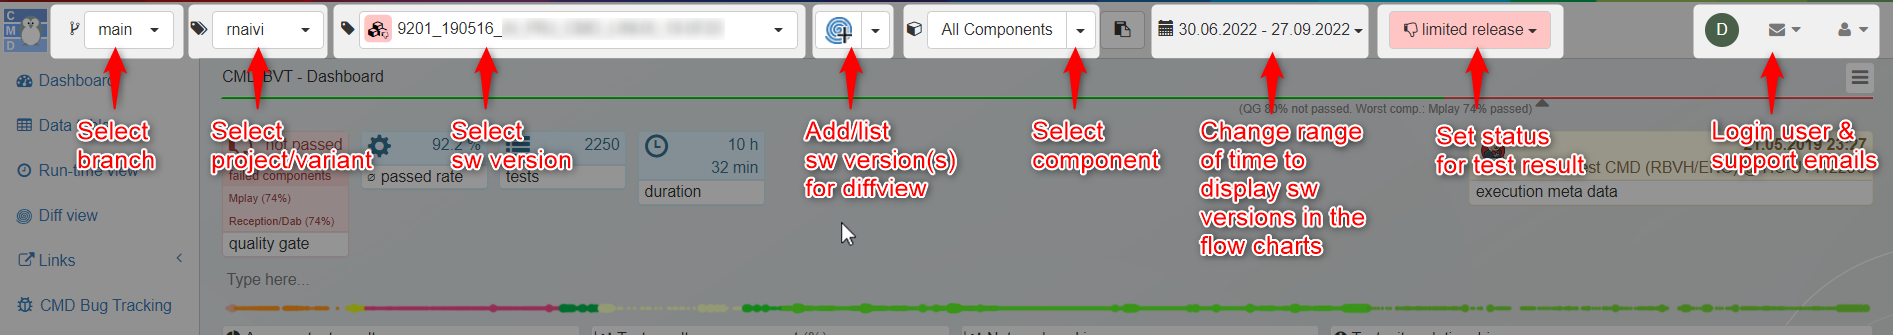
\includegraphics[width=1\linewidth]{./pictures/main-menu.png}

\hypertarget{dashboard-view}{%
\subsection{Dashboard View}\label{dashboard-view}}
The Dashboard view does not only provide an overview of test execution results but 
also shows the correlation betweeen components within the result and relationship with other test execution results.

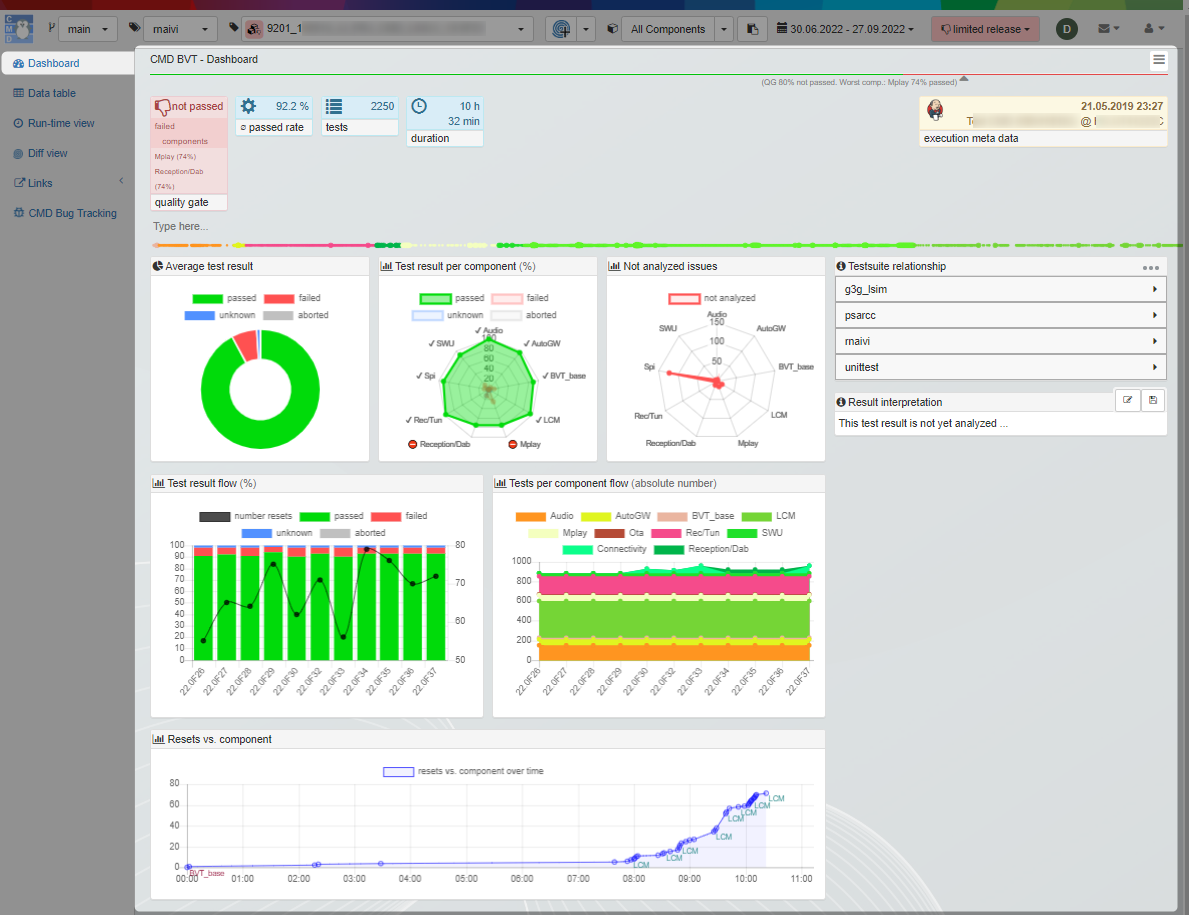
\includegraphics[width=1\linewidth]{./pictures/view_dashboard.png}

\subsubsection{Result overview}
At the top left corner of the Dashboard view you find the test execution result 
statistics:

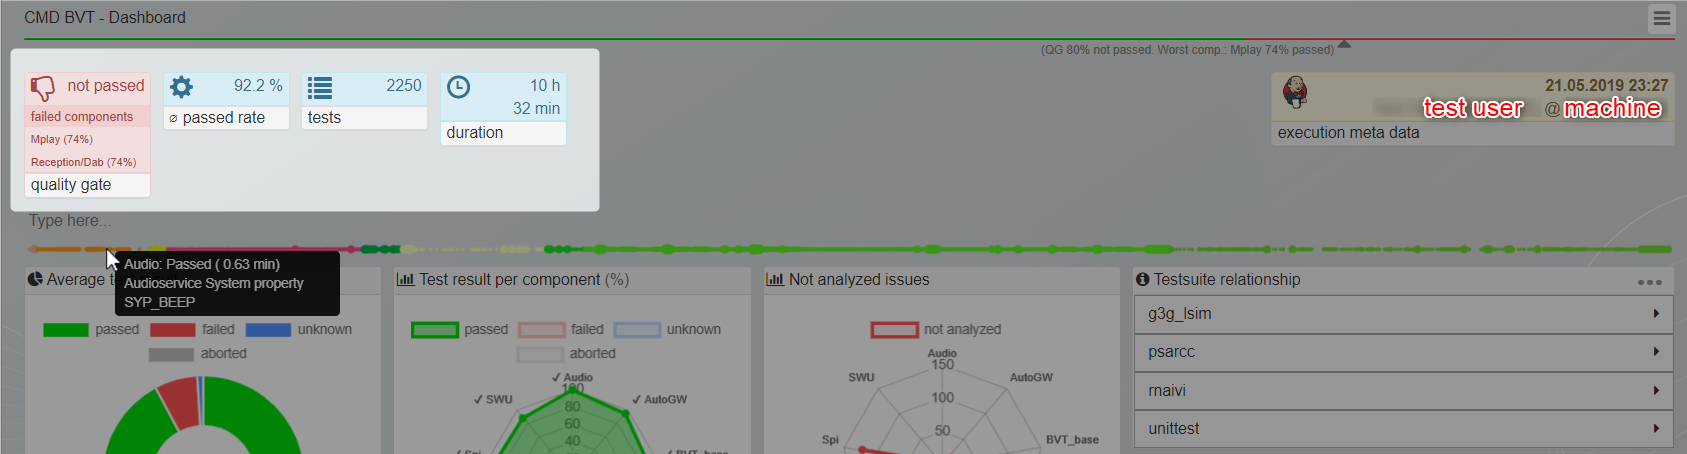
\includegraphics[width=1\linewidth]{./pictures/dashboard/result_statistics.png}

Which contains:
\begin{itemize}
   \item Overrall status (you can define a qualitiy gate).
   \item Passed rate.
   \item Total number of executed test cases.
   \item Test execution duration.
\end{itemize}

On other right-hand side, there is information about the execution environment:

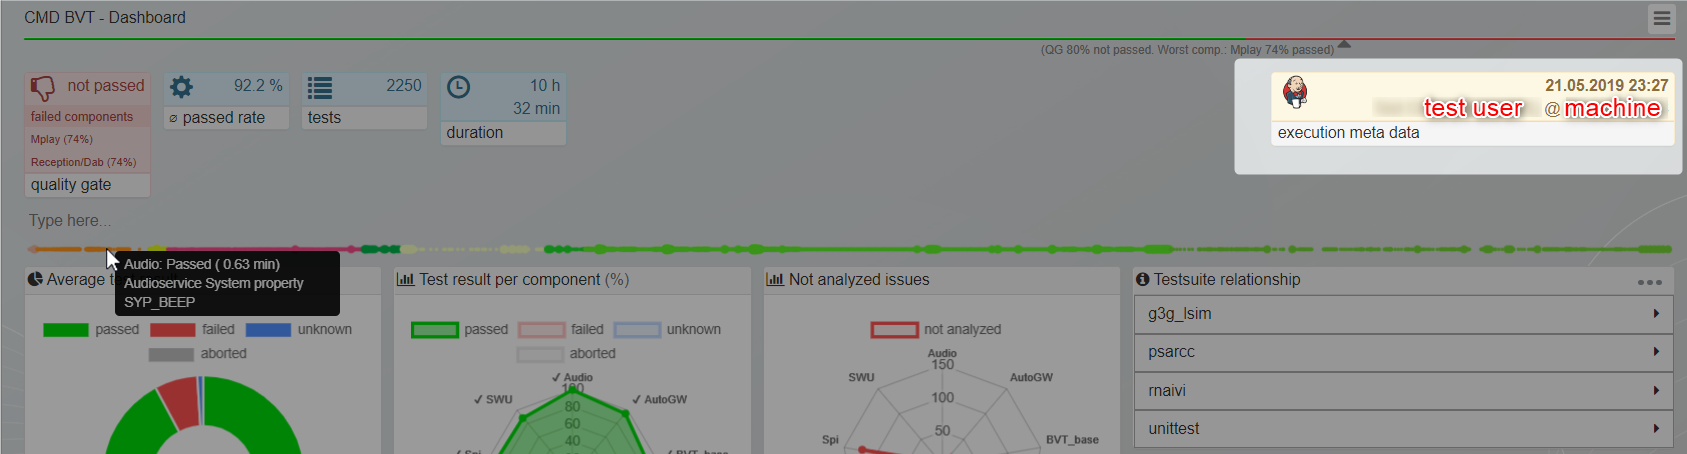
\includegraphics[width=1\linewidth]{./pictures/dashboard/result_environment.png}
\begin{itemize}
   \item Execution time (start of test execution)
   \item Test machine
   \item Test user
   \item Jenkins link (embedded URL in the Jenkins's icon)
\end{itemize}

Below them is the test execution result timeline:

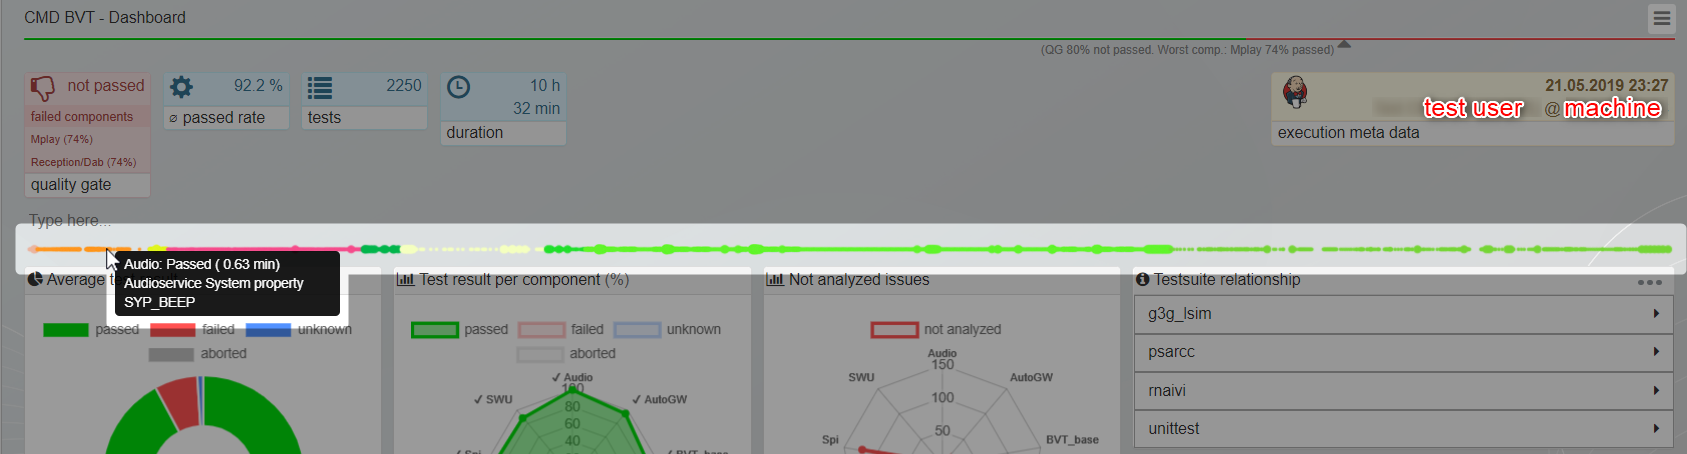
\includegraphics[width=1\linewidth]{./pictures/dashboard/result_timeline.png}

It provides:
\begin{itemize}
   \item The timeline of the executed test cases which are grouped by components 
         (different color). Left side is start of testing. Right side the end.
   \item How much time is consumed by the individual test case by the distance 
         to the next test at the time line or the detail pop-up when hovering on the 
         dot at the timeline.
   \item Test status result: A small dot for \ifpassed{Passed} status and a big dot 
         for others.
\end{itemize}


The next \textbf{Average test result} chart will give you the detail of the test 
result with the percentage (number of test cases will be shown when moving the mouse 
over the pie chart) of each result status (\ifpassed{Passed}, \iffailed{Failed}, 
\ifunknown{Unknown} or \ifaborted{Aborted}) of the execution. 

So that, you can qualify this test execution result is good or not.

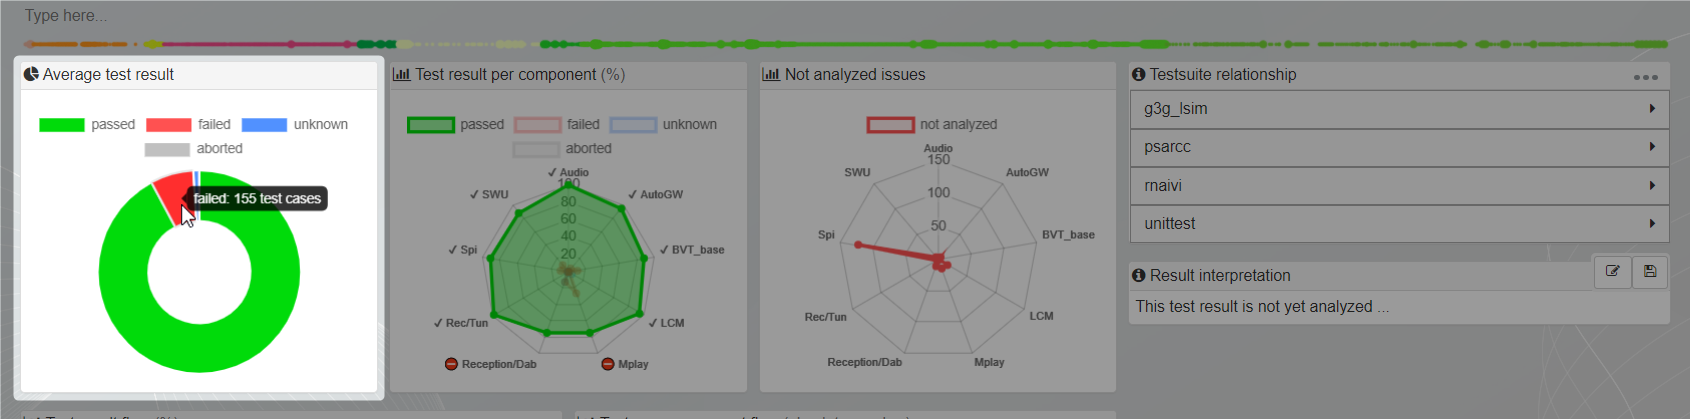
\includegraphics[width=1\linewidth]
{./pictures/dashboard/chart_average_test_result.png}

\subsubsection{Component's correlation}
The next charts will help you to get the correlation between components within
the test result, so that you can know which component(s) impact(s) the test
result.

\textbf{Test result per component} chart: provides a fast overview of 
test result percentages over all components. Here you can quickly see
the quality of the system under test. Idially the spider chart should
be fully green. This means that all component tests result in 100\% \ifpassed{Passed}.

You can also define a quality gate (default 80\%) which results in a "minus"
in front of the component name if the quality gate is not reached.


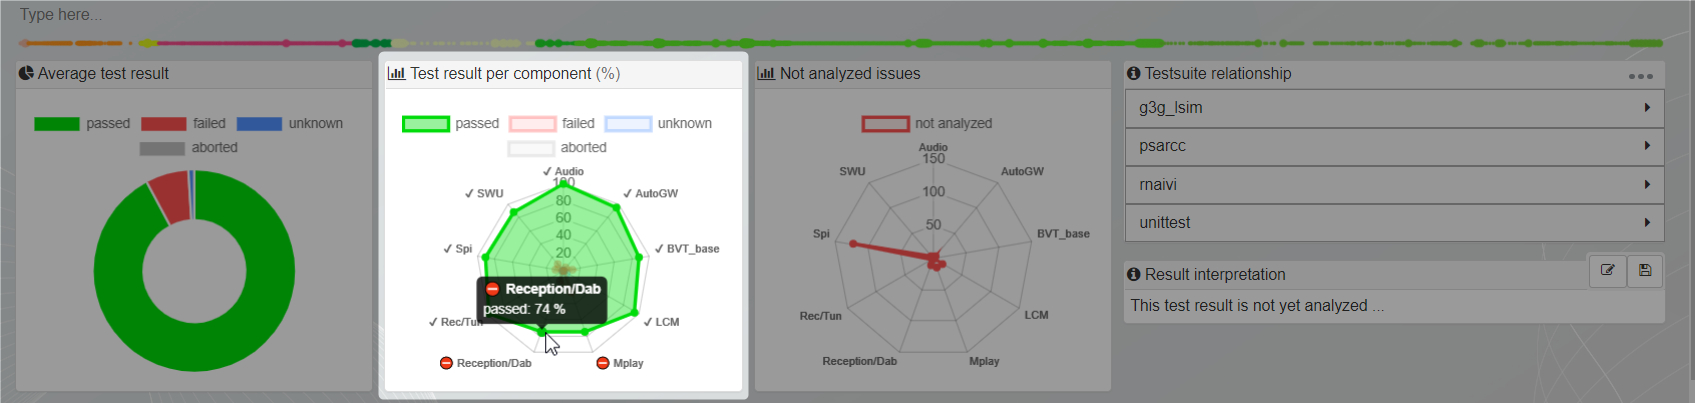
\includegraphics[width=1\linewidth]
{./pictures/dashboard/chart_test_result_per_component.png}


\textbf{Not analyzed issues} chart: you can known how many test cases of 
components are issued without analysis. 

The Datatable view provides a process to set \iffailed{Failed} test cases to
"analyzed". Ideally this spider chart should have a red dot in the center.
This means all \iffailed{Failed} test cases are analyzed.

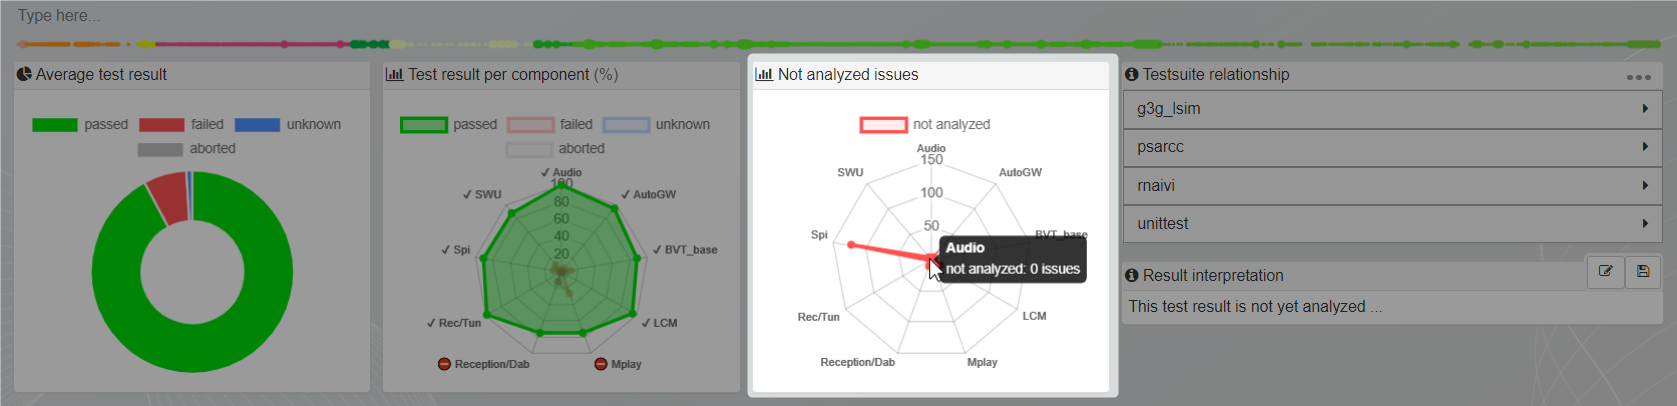
\includegraphics[width=1\linewidth]
{./pictures/dashboard/chart_not_analyzed_issues.png}

\subsubsection{Relationships with other test execution results}

- \textbf{Testsuite relationship}: will let you know all the related test 
results (grouped by project/variant) of the current selected version.

This allows to quickly go to related test results to have a fast comparison
about the quality of the selected version across all projects/variants.

\underline{For example:} the selected version have been executed for 4 
projects/variants: \emph{g3g\_lsim}, \emph{psarcc}, \emph{rnaivi} and 
\emph{unittest}. Each variant (except the \emph{unittest}) has 2 test results 
(one for the smoke test and one for the whole test execution result).

Then, all the related test execution results will be displayed as below:

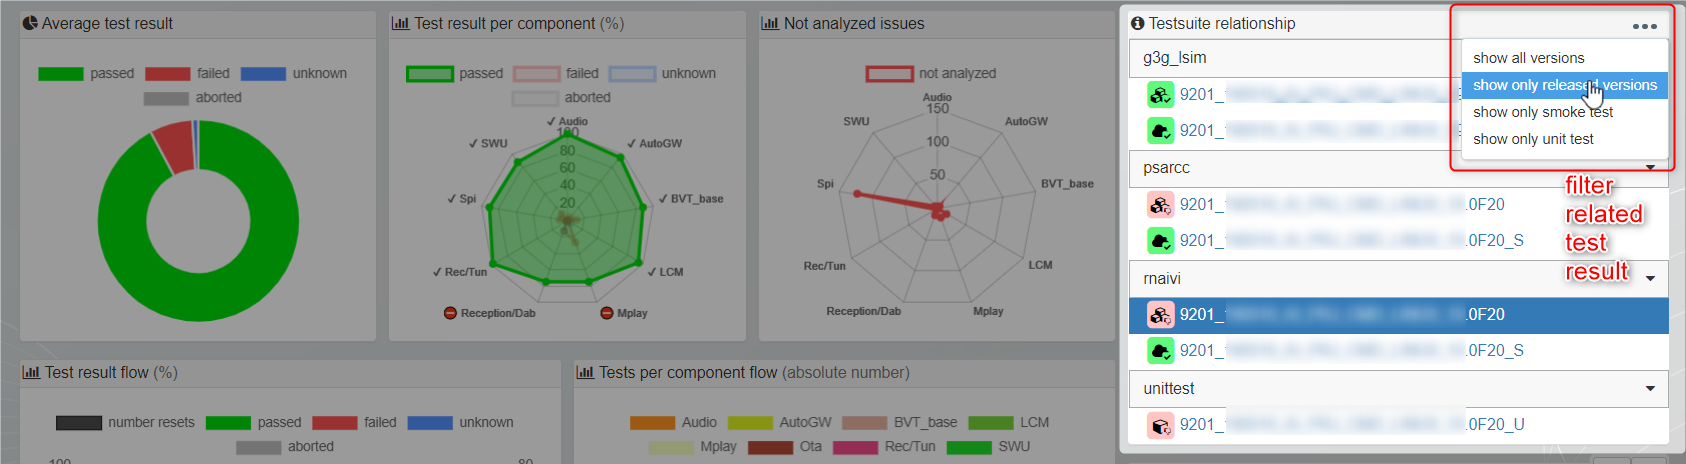
\includegraphics[width=1\linewidth]
{./pictures/dashboard/testsuite_relationship.png}

There is also the context menu (\textbf{...}) that allows you to filter the 
related test results.

- \textbf{Test result flow} chart: provides the picture of quality change 
(percentages of each status) between versions. 

So that, you can understand the quality of testing software is being improved 
or vice versa.

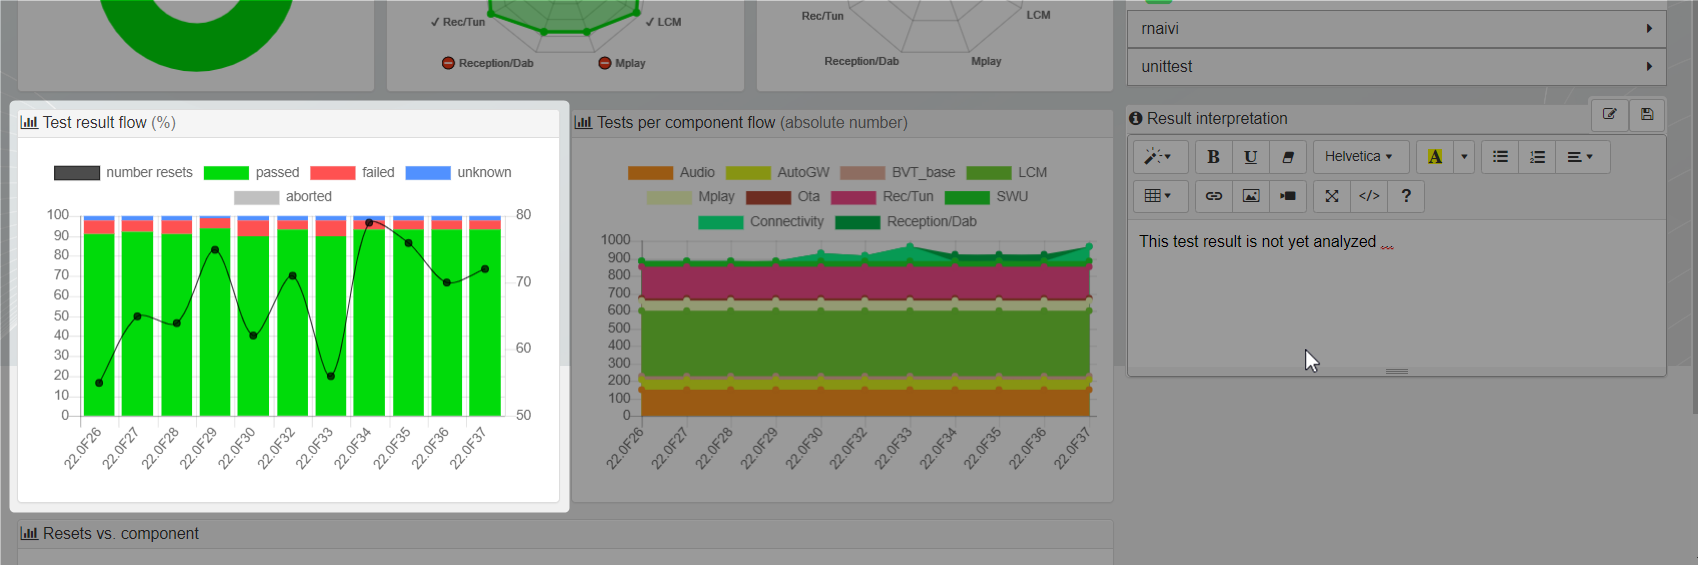
\includegraphics[width=1\linewidth]
{./pictures/dashboard/chart_test_result_flow.png}

- \textbf{Tests per component flow} chart: provides the change of number test
cases per component between versions.

You can aware the number of test cases per component and how many test cases are
added or removed (per component or the whole test result) from those versions.

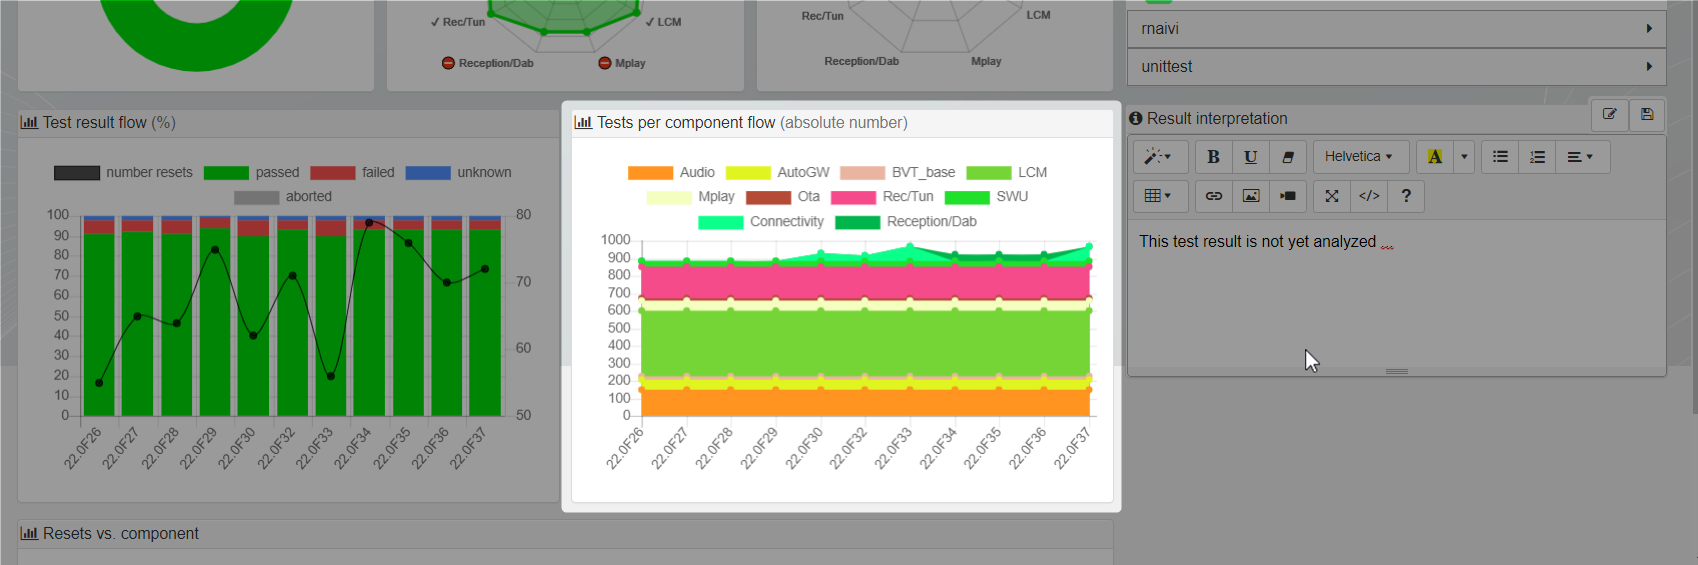
\includegraphics[width=1\linewidth]
{./pictures/dashboard/chart_tests_per_component_flow.png}

\begin{boxhint}{Notice}
The versions which are displayed in \textbf{Test result flow} and 
\textbf{Tests per component flow} charts are the executed test results within 
the selected range of time in 
\hyperref[main-menu]{the main menu} (default is \textbf{Last 90 Days}).
\end{boxhint}

\subsubsection{Result interpretation}
You can give more information, provide an analysis, take notes, ... on the 
execution result by leaving comments in the \textbf{Result interpretation} 
section.

As soon as the comment(s) is saved, that information will be updated to 
the database. So that, other users who browse to this test result can see
the analysis/comment for reference.

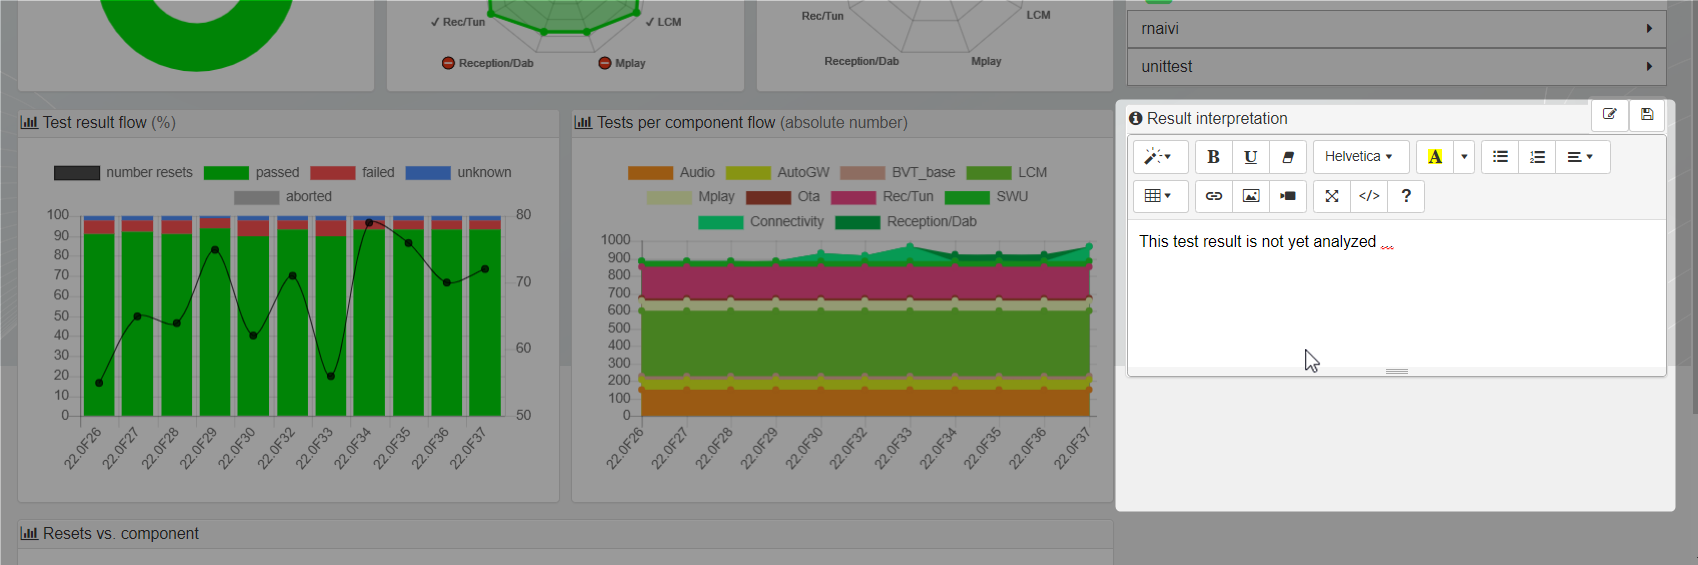
\includegraphics[width=1\linewidth]
{./pictures/dashboard/result_interpretation.png}

\subsubsection{Resets vs. component}

The \textbf{Resets vs. component} chart will helps you to know the interaction
of component with the DUT (device under test) by providing the the reset counter
per component during the execution.

You can have awareness that:
\begin{itemize}
   \item When DUT has been reset.
   \item Which component has reset the DUT.
   \item How many reset has been done during each component and the whole
         test execution.
\end{itemize}

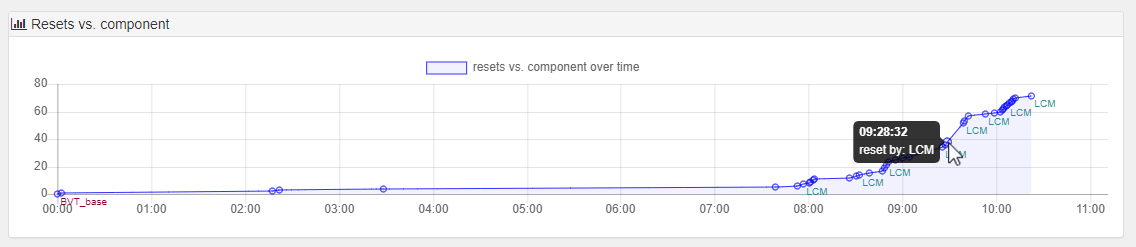
\includegraphics[width=1\linewidth]
{./pictures/dashboard/reset_vs_component.png}

\hypertarget{datatable-view}{%
\subsection{DataTable View}\label{datatable-view}}

Datatable view provides the summary table which contains the detail information 
of each test case (grouped by component) within the test execution.

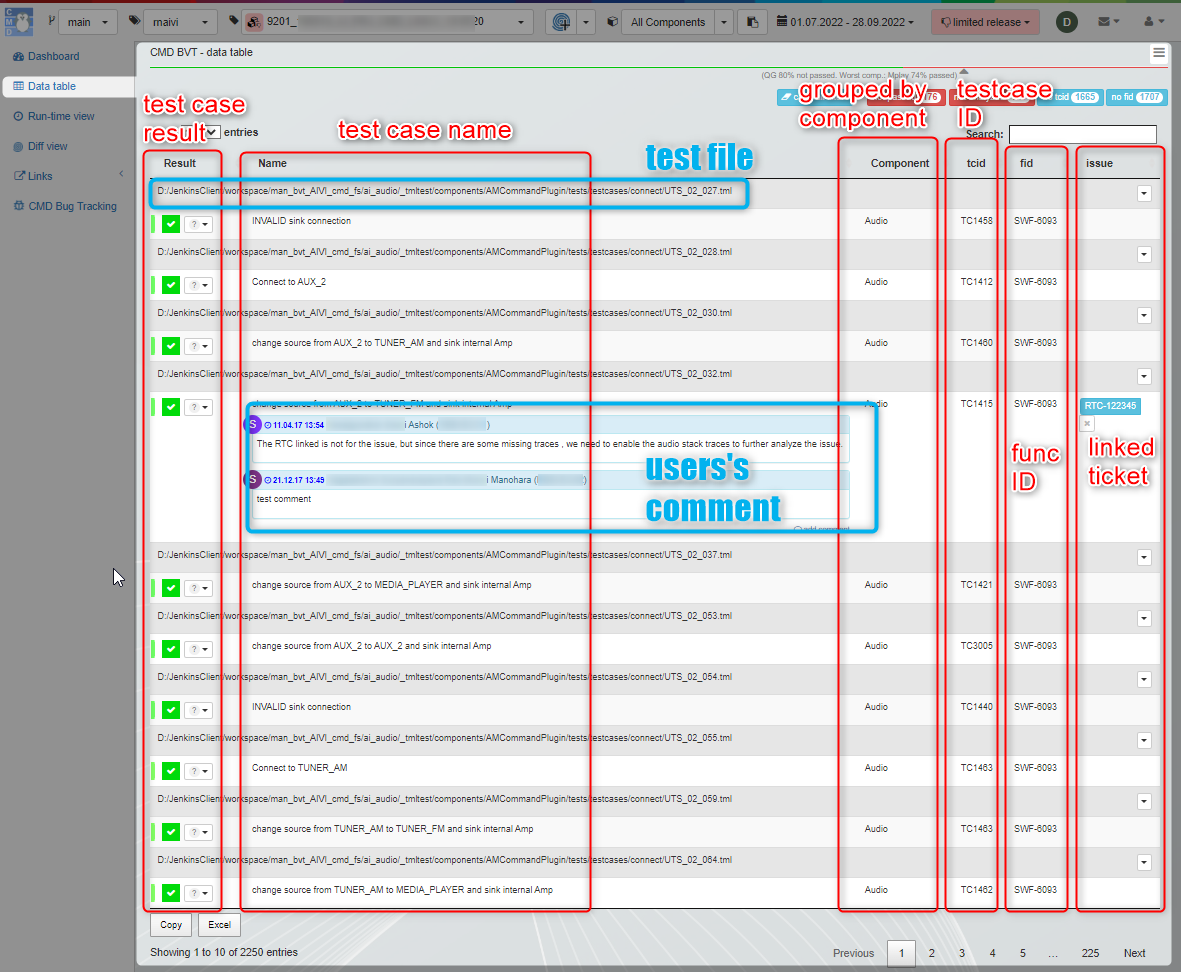
\includegraphics[width=1\linewidth]{./pictures/view_datatable.png}

Besides, you can aslo:
\begin{itemize}
   \item determine how many test cases (entries) are displayed in the table page.

         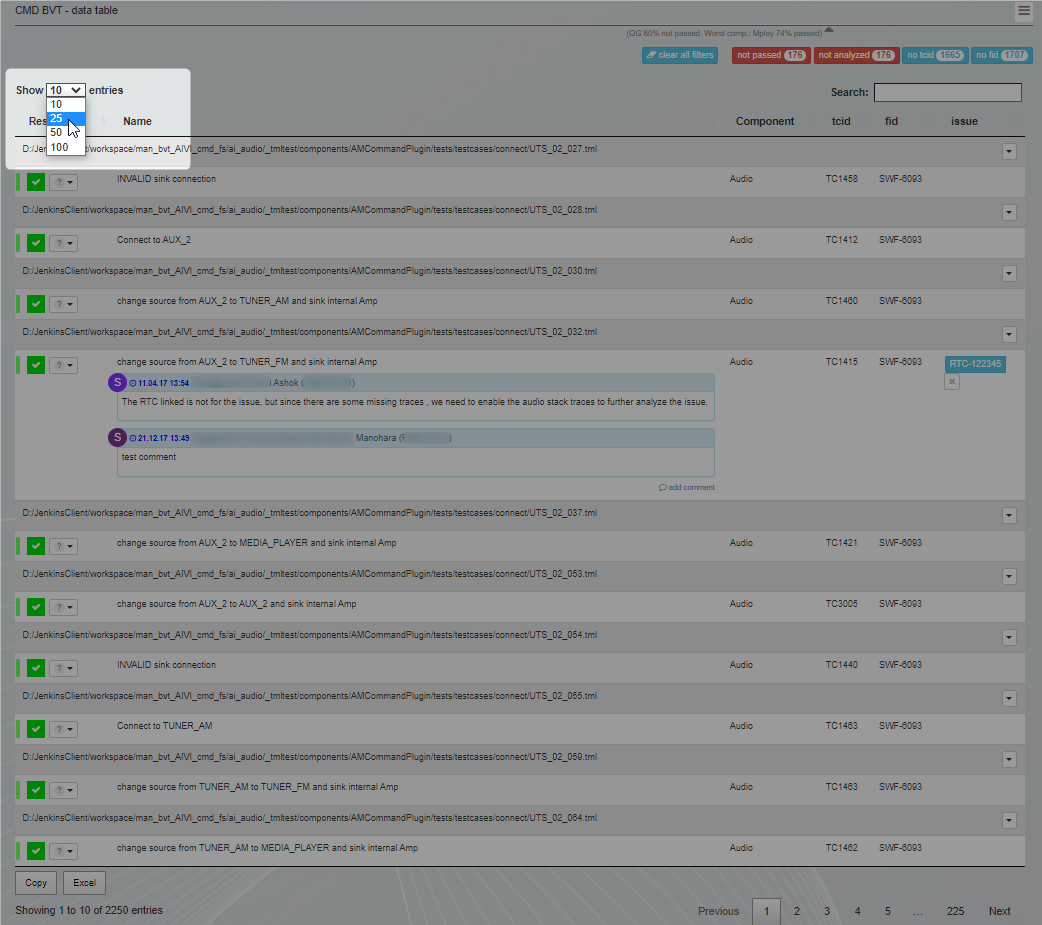
\includegraphics[width=0.6\linewidth]
         {./pictures/datatable/change_number_entries.png}
         
   \item apply filters to display such as not \ifpassed{Passed} test cases.
   
         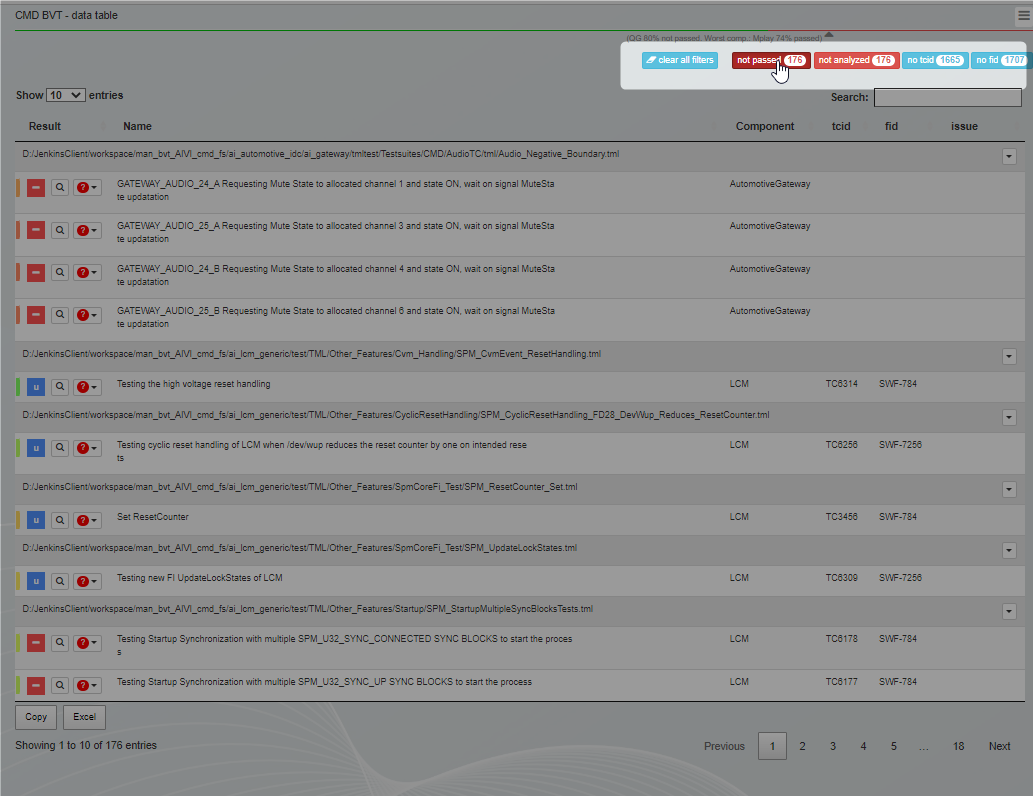
\includegraphics[width=0.6\linewidth]
         {./pictures/datatable/apply_filter.png}

   \item search for the specific test case for reference.
   
         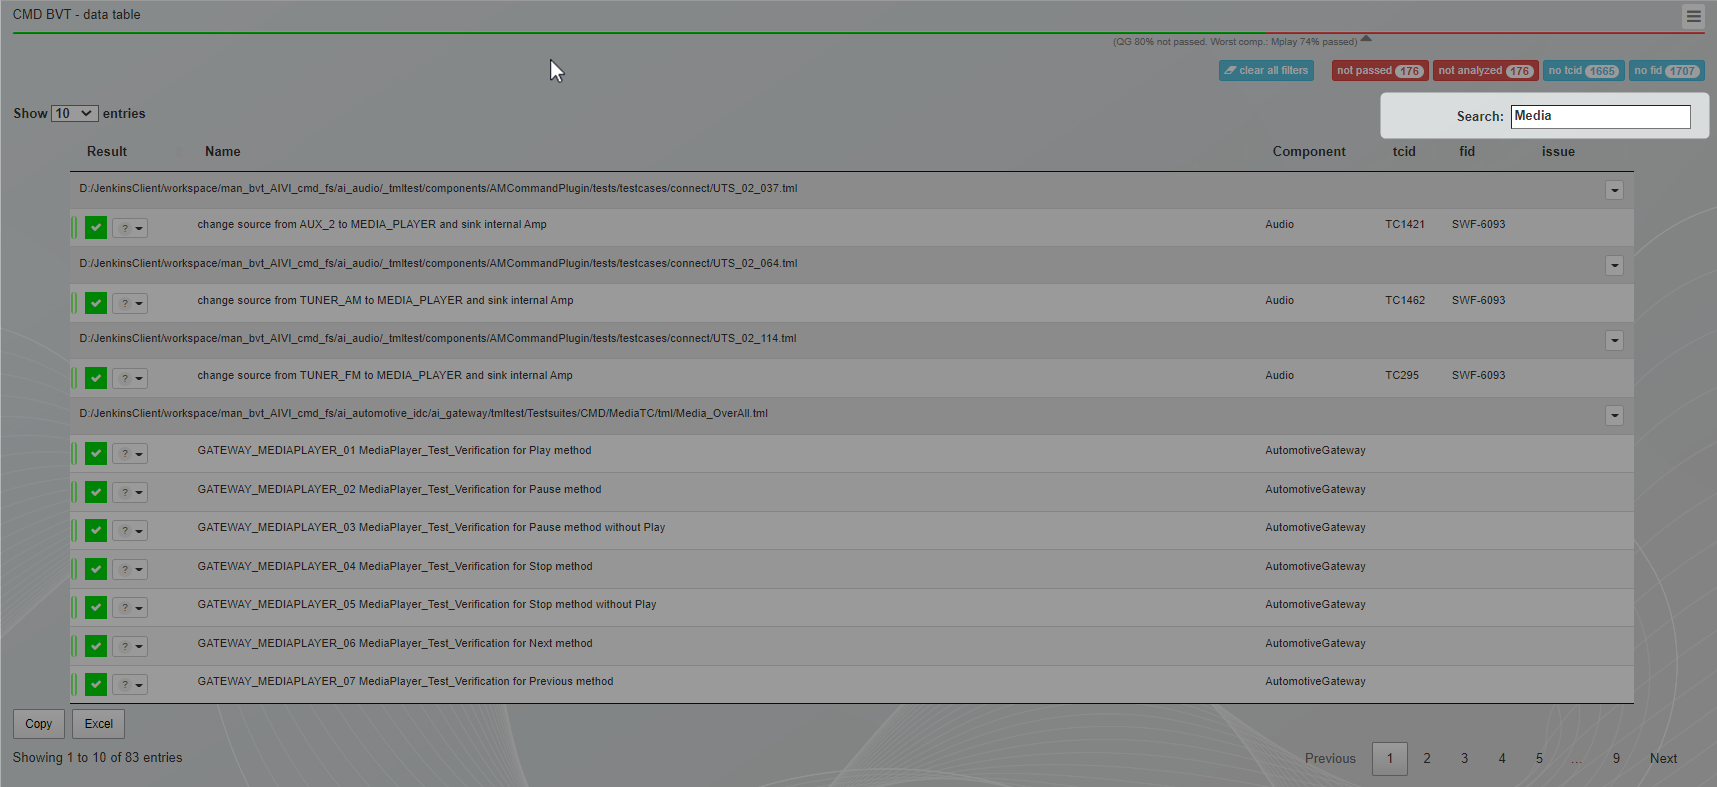
\includegraphics[width=0.6\linewidth]{./pictures/datatable/search.png}

   \item get more information about test environment, configurations.
   
         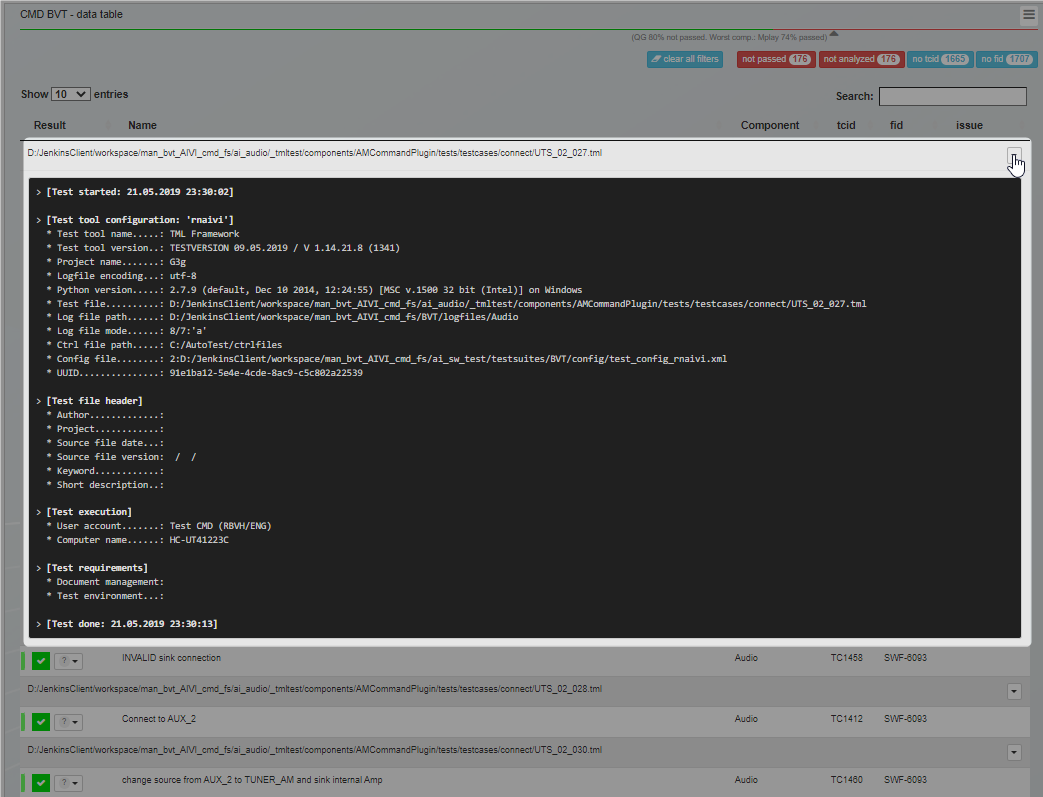
\includegraphics[width=0.6\linewidth]
         {./pictures/datatable/testcase_detail.png}

   \item get traceback information for not passed test case(s). An pop-up will 
         be displayed which show all record traceback (error) information.

         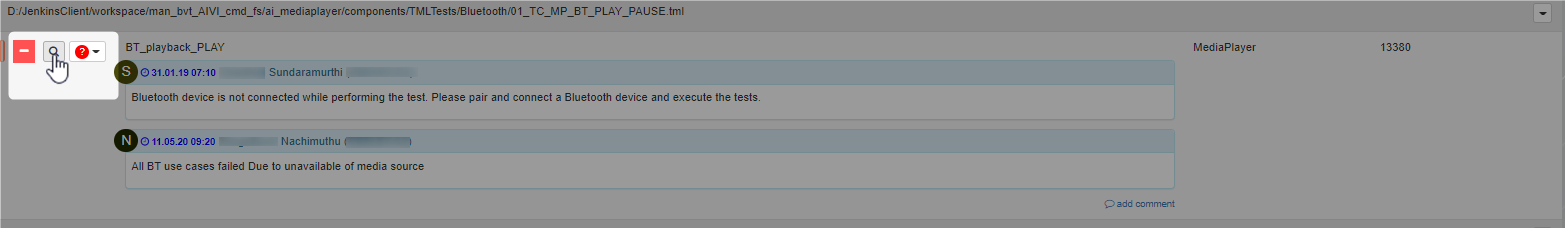
\includegraphics[width=0.6\linewidth]
         {./pictures/datatable/testcase_traceback.png}

   \item give comment to test case, link issue ticket to test case or observe
         the history of the user interaction on the test case.

         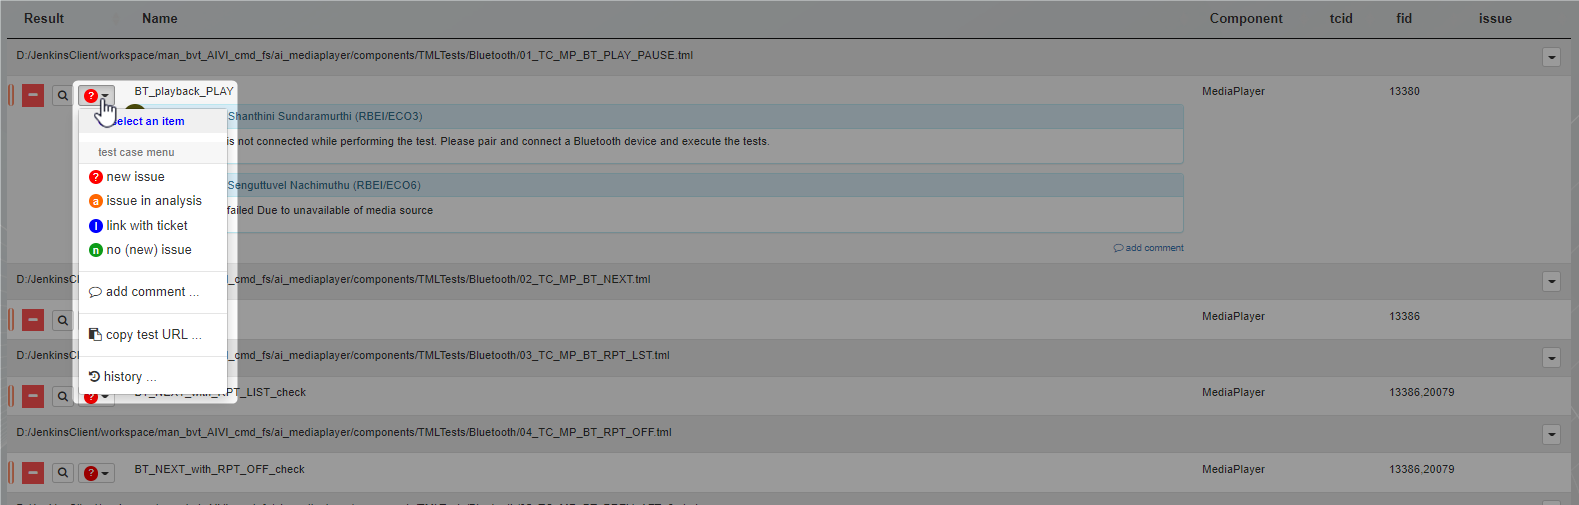
\includegraphics[width=0.6\linewidth]
         {./pictures/datatable/testcase_menu.png}

   \item copy data table or export them to the excel file.

         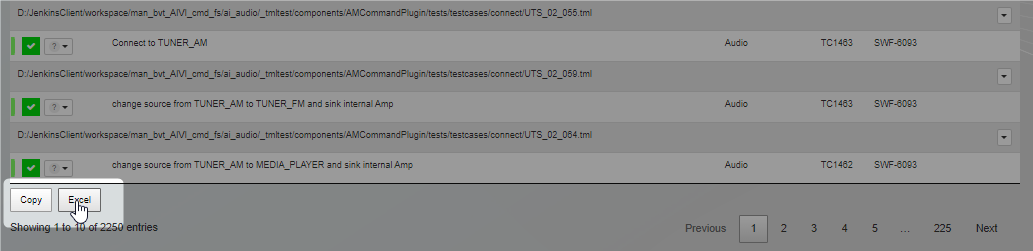
\includegraphics[width=0.6\linewidth]
         {./pictures/datatable/copy_export.png}
\end{itemize}


\hypertarget{runtime-view}{%
\subsection{Runtime View}\label{runtime-view}}
The runtime provides the treemap chart which helps you to know the runtime of 
components within test execution result or test cases within each component.

You can click on the component to go to detail runtime of all test cases within 
it and go back by clicking the component header.

With this view, you can understand the runtime of a your test suite then 
optimize the specific component or testcase if required.

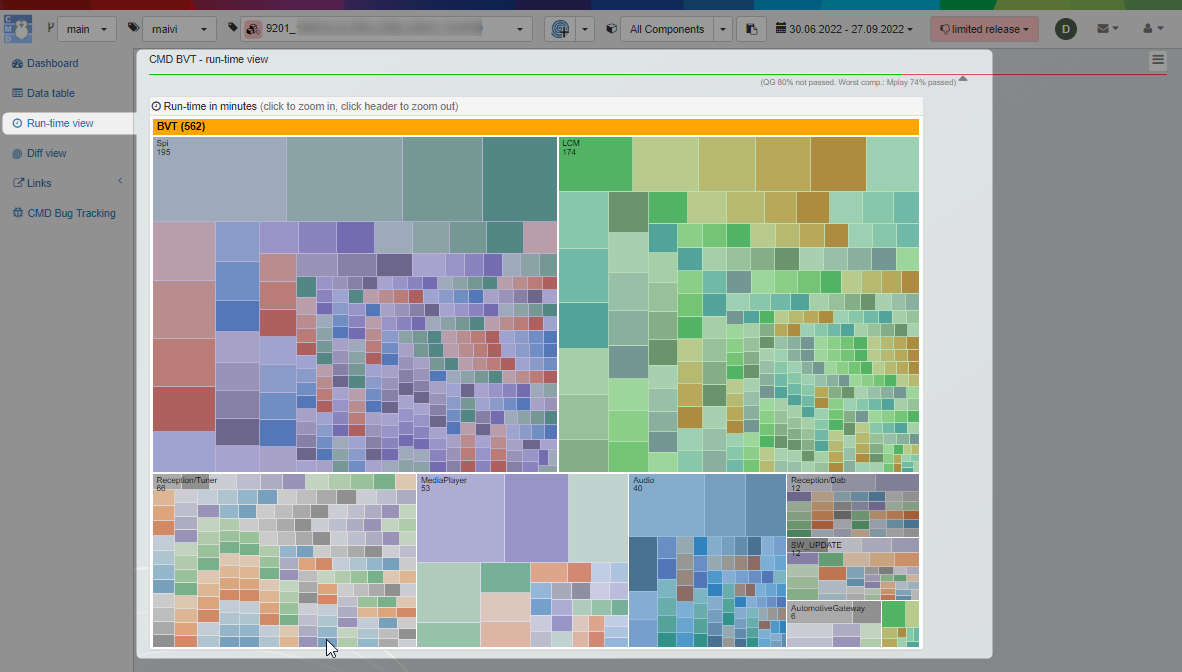
\includegraphics[width=1\linewidth]{./pictures/view_runtime.png}

\hypertarget{diff-view}{%
\subsection{Diff View}\label{diff-view}}
The diffview contains only the spiral chart which displays the differences 
between the software versions you want to compare. So that you can:
\begin{itemize}
   \item observe the test case result change (e.g from \ifpassed{Passed} to 
         \iffailed{Failed}).
   \item aware the new or removed test case(s).
   \item recognize the unstable test case(s)/component(s).
\end{itemize}

Be default, without adding the version for diffview, the current selected 
version and its around versions (the previous and the next version if existing) 
will be chosen for diffview as below:

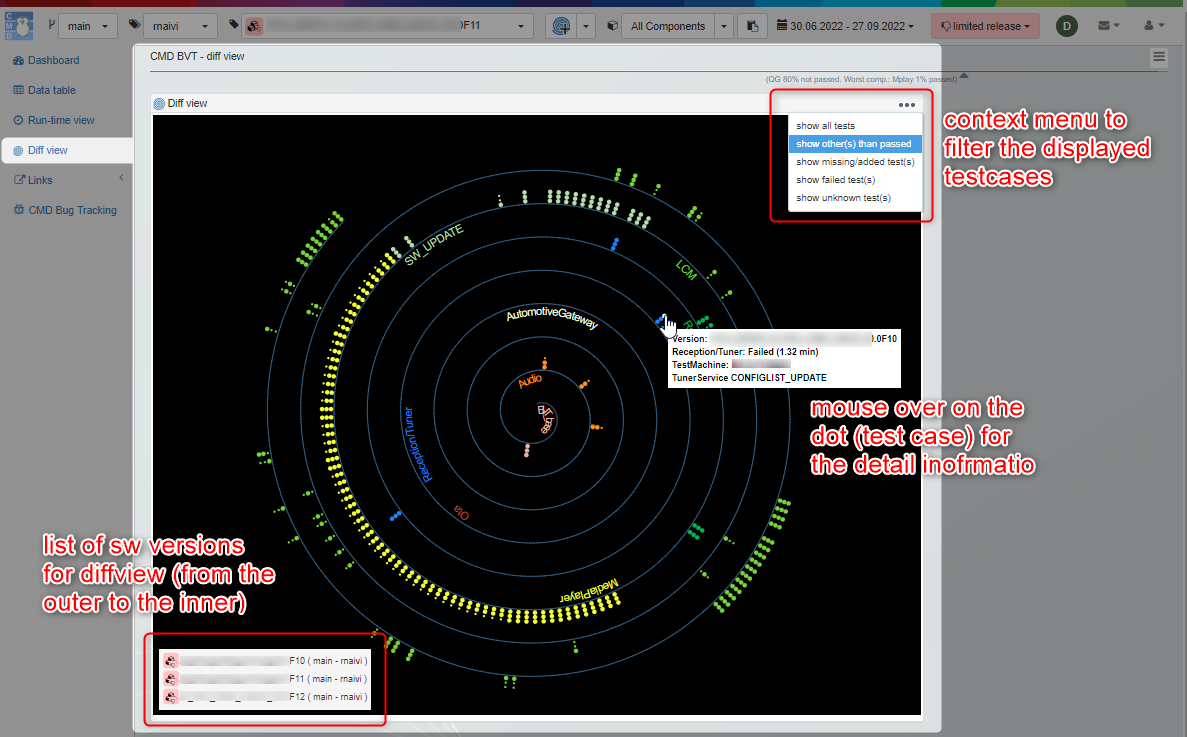
\includegraphics[width=1\linewidth]{./pictures/diffview/default_detail.png}

In case, you want to add the specific versions for diffview, select the version
from the version select box then click the add button 
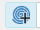
\includegraphics{./pictures/diffview/add_button.png}
to add it to the list of diffview. 

The next dropdown button is used for viewing your selected versions.
You can also clear your selection with \textbf{clear list} option.

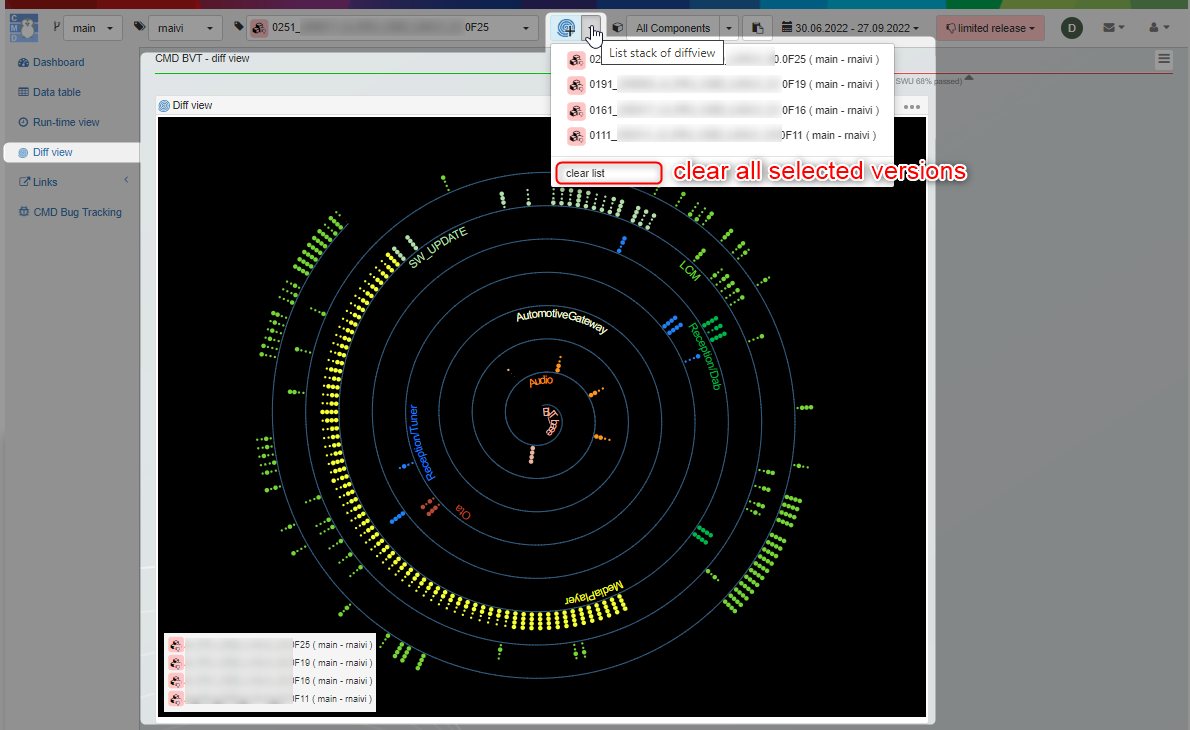
\includegraphics[width=1\linewidth]{./pictures/diffview/selected_version.png}

As soon as the new version is added for diffview, the spiral chart is updated 
immediately.

The dots which present for the test cases along the spiral line (small dot is 
\ifpassed{Passed} and bigger one for other status) are interactable. 
It means that you can:
\begin{itemize}
   \item mouse over the dots to see the test case information.
   \item click on the failed test case (bigger dot) for the traceback 
         information.
\end{itemize}

\begin{boxhint}{Notice:}
   You can only select maximum of \textbf{5} versions for diffview.

   If the maximum of selected versions is reached and you click on the button to 
   add more, the warning message will be displayed to prevent that action.
\end{boxhint}

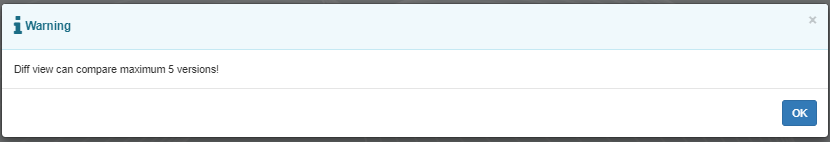
\includegraphics[width=1\linewidth]{./pictures/diffview/warning.png}

\hypertarget{developer-guidance}{%
\section{Developer guidance:}\label{developer-guidance}}

\begin{boxhint}{Notice:}
In order to run up the TestResultWebApp, it requires some knowledge about:
\begin{itemize}
   \item Web server: setup and run web server for web hosting.
   \item Nodejs platform and Express framework: adapt the sourcecode with your
         environemnt: domain, configurations, ...
   \item Mysql database: schema, tables, SQL scripting. We propose to use 
         \href{https://dev.mysql.com/doc/workbench/en/}{MySQL Workbench} tool
         for working with Mysql database.
\end{itemize}
\end{boxhint}

\subsection{How to run new TestResultWebApp instant:}
\begin{enumerate}

\item Precondition:
\begin{itemize}
\item \href{https://nodejs.org/en/}{Nodejs} shoulde be installed.
\item \href{https://dev.mysql.com/downloads/mysql/}{mysql server} should be 
      installed.
\item A cloned package's resource from 
      \href{https://github.com/test-fullautomation/testresultwebapp}
      {Github repo}
\begin{robotlog}
git clone https://github.com/test-fullautomation/testresultwebapp.git
\end{robotlog}
\item The port which will run nodejs application (default is \textbf{3000}) is
      opened (enable) in firewall.

\end{itemize}

\item Setup mysql database:
\begin{itemize}
\item create \emph{user}, \emph{password} and \emph{schema} then update them  
      as \rcode{global.mySQLOptions} in  \\
      \rlog{webapp/web_server/lib/global.js} file.
\item create required tables in your database schema with MySQL Workbench.
\begin{itemize}
\item open the datamodel which is located at
      \rlog{mysql\_server/datamodel/test\_result.mwb}
\item export all defined tables in datamodel to your schema, use 
      \textbf{Foreward Enginneer to Database} feature of MySQL Workbench.
\begin{robotlog}
EER Diagram > Database > Forward Engineer... > your schema
\end{robotlog}
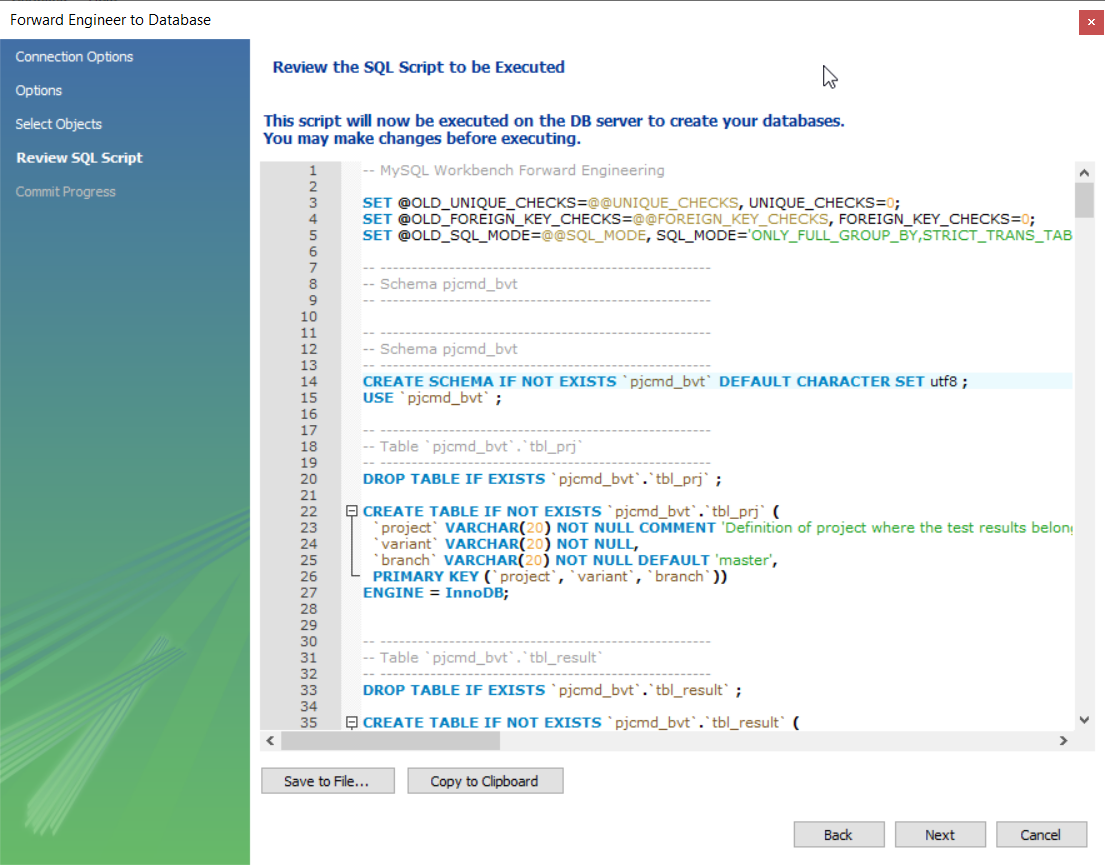
\includegraphics[width=1\linewidth]{./pictures/forward_engineer.png}
\begin{boxhint}{Notice}
If you have created your schema with other name than the default 
name \emph{pjcmd\_bvt}, you should replace the schema name at the \textbf{Review
SQL Script} step:
\begin{itemize}
\item copy SQL script to text editor such as VsCode
\item replace \emph{pjcmd\_bvt} which your new schema name
\item paste SQL script back to the \textbf{Foreward Enginneer to Database} 
      tool
\end{itemize}
before moving to next step to execute SQL script.
\end{boxhint}

\item create all store procedures by loading all SQL scripts under 
      \rlog{mysql_server/TMLdb_sproc/} folder then execute them.

\begin{boxhint}{Notice}
If you have created your schema with other name than the default 
name \emph{pjcmd\_bvt}, you should replace the schema name before executing SQL 
scripts.
\end{boxhint}

\end{itemize}

\end{itemize}

\item Import the initial data to the database with \href{https://github.com/test
-fullautomation/robotframework-testresultwebapptool}{RobotResults2DB tool}.

\item Adapt Web server:
\begin{itemize}
   \item \rlog{web_server/lib/global.js}: for domain, database's configuration,
         keys for authentication, ldap server for authentication, ...
   \item \rlog{web_server/test.js}: for listening port of nodejs application.
\end{itemize}

\item Adapt Web client:
\begin{itemize}
   \item \rlog{web_client/dashboard/dist/js/common/global.js}: for domain.
   \item \rlog{web_client/dashboard/dist/js/common/communication.js}: for 
         listening port of nodejs application's API.
\end{itemize}

\item Start nodejs application by command:
\begin{robotlog}
node testdb.js
\end{robotlog}

\item Start web server for hosting the static files:

You can use any web server \href{https://httpd.apache.org/}{Apache}, 
\href{https://www.iis.net/}{IIS} or \href{https://www.nginx.com/}{Nginx} for 
hosting the static files under \rlog{web_client/dashboad/} folder when running 
as production.

For development, you can use directly \rlog{express.static} which is supported 
by Express framework for hosting static files.
The \rlog{web_server/test.js} file should be modified to add this setting.

\begin{robotcode}[linebackgroundcolor=\hlcode{4,10}]
'use strict';

var global = require('./lib/global');
var path = require('path');

...

//for local GUI tests deliver static HTML 
//content from port 3000
app.use(express.static(path.join(__dirname, "../web_client/dashboad/"))); 

var session = require('express-session');
var MySQLStore = require('express-mysql-session')(session);
...
\end{robotcode}

\item Now open your favourite browser, go to the domain of webapp and enjoy.

\end{enumerate}
